\newpage

\chapter{Introduction}
Argumentation is increasingly becoming a popular aspect of Artificial Intelligence that deals with the creation of knowledge systems and evaluation of decision problems. Past and current research has allowed for the development of various argumentation frameworks that allow the analysis of arguments by formulating them in a formal manner and evaluating them. This project focuses mostly on Assumption-Based Argumentation (ABA) and its implementation through a practical argumentation system.  ABA is a form of argumentation where arguments and attacks are notions derived from primitive notions of rules in a deductive system, assumptions and contraries thereof \cite{abatut}.  This framework allows for the evaluation of a conclusion based on whether it is supported by a ``winning'' set of arguments. Such sets of arguments and assumptions can be determined as ``winning/acceptable'' based on a number of different semantics that ABA supports, which are discussed in more detail later on in the report. 

Therefore, ABA is a potentially powerful tool which one could use to establish the validity of the conclusion put forward. Early successful application of argumentation theory and the ABA framework have occurred in fields such as legal-reasoning, medical diagnosis and decision theory. Within these fields ABA has been used not only because of its ability to determine propositions as acceptable, but also due to its ability to convey the derivation process to the user. There are various computational mechanisms that have been devised to algorithmically compute the acceptability of a claim. Using these mechanisms argumentation engines, such as proxdd \cite{proxdd} and grapharg \cite{grapharg}, have been implemented thus allowing for the computation of acceptability of a claim under a defined ABA framework. Nonetheless, these engines are still at a primitive stage and require enhancing for ABA to become a widely accepted and applied tool in the real world.

Namely, there is a lack of an application that is easily accessible to users and provides both satisfactory performance and useful visualisations of the argument. The difficulties involved with creating such an application are multifold.  These involve the performance of the underlying engine when dealing with large scale real problems, the difficulty a user might face in devising a correct ABA framework for their problem and devising a visualisation system to accurately convey the derivation process to the user. Additionally, the engines themselves are still at an early stage and need to be extended. For example the proxdd and grapharg systems lack the ability to derive the acceptability of a claim based on ``ideal'' semantics. Lastly, there is a lack of generalisation of these systems. At their current state they aim at simply resolving ABA frameworks directly implemented into the engine. This restricts the usability of the system to users who intend to use just ABA and have significant knowledge of ABA to device the initial framework of their problem.

The project's objectives centre around providing solutions to the problems mentioned above by fulfilling the requirement for a web-based argumentation application that will allow users to exploit the existing ABA systems. The web-application should act as a platform that will provide the users with good user experience and the ability to easily and as seamlessly as possible interact with the ABA systems in the back end. Having computed the necessary derivation the user will be provided with the output in a useful and meaningful manner in the form of a visualisation. The end system would be similar to the ASPARTIX system implemented by TU Wien \cite{aspartix}. Having established the web-application, the project will then seek to enhance the existing systems by enabling them to compute based on more semantics mentioned above. Potentially the project might look in the development of a simple API for these engines. Lastly, the web-application might be extended to support Abstract Argumentation through its mapping to ABA (as described by \cite{AAmapping}) and allow the direct input of decision problems (as described in \cite{decision}). 

\section{Incorporating derivation engines in a web application.}

We looked into designing a web application that would provide an online interface to the derivation engines. This includes a clean and simple interface by which the user is able to choose both the engine and the semantics required and would also allow them to define their ABA framework. Figure [TODO] provides a screen shot of the GUI used by the user to interact with the derivation engines. The implementation and design choices are detailed in sections [TODO].

\begin{figure}[h]
    \centering
    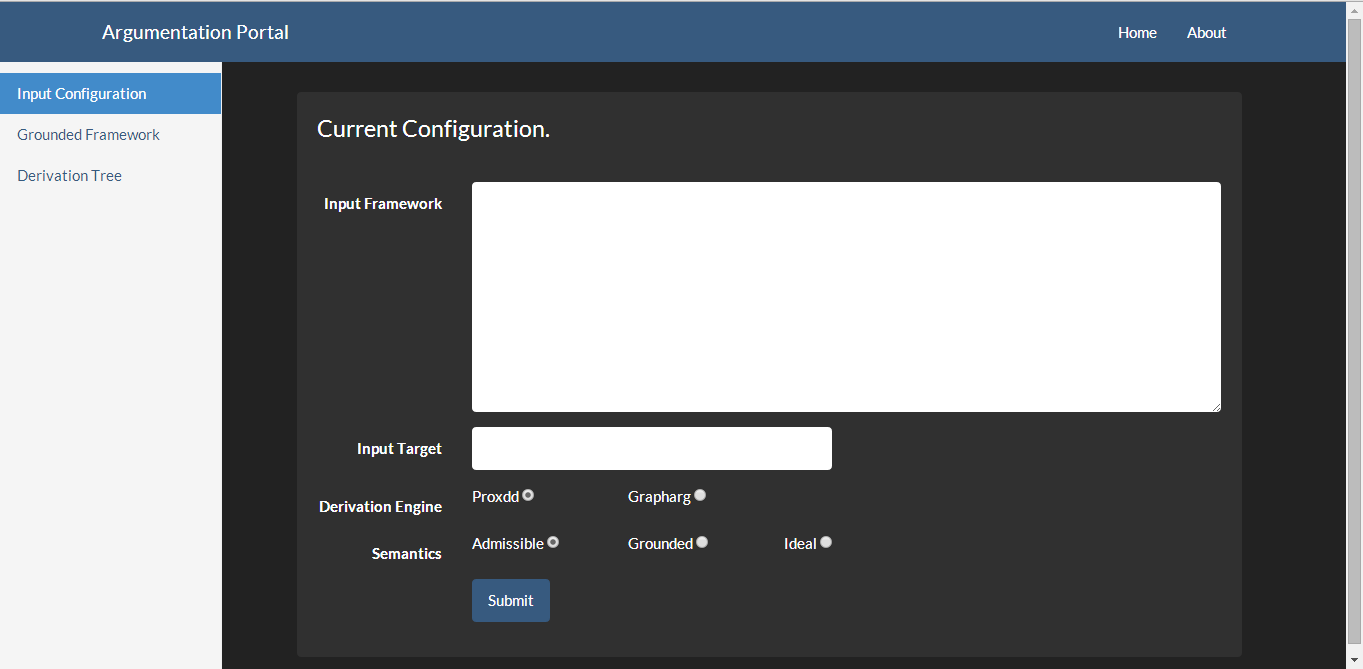
\includegraphics[width=0.8\textwidth]{argumentationInput.png}
    \caption{Input configuration panel.}
    \label{fig:arg_config}
\end{figure}

\section{Visualising the derivation trees.}

We then looked into a suitable output method of the solution received from the derivation engines. This involves the visualisation of the derivation tree on a canvas environment as illustrated in figure [TODO]. The visualisation provides a clear and concise method for the user to evaluate the derivation of the claim they submitted. The implementation of the visualisation is discussed further in section [TODO].

\begin{figure}[h]
    \centering
    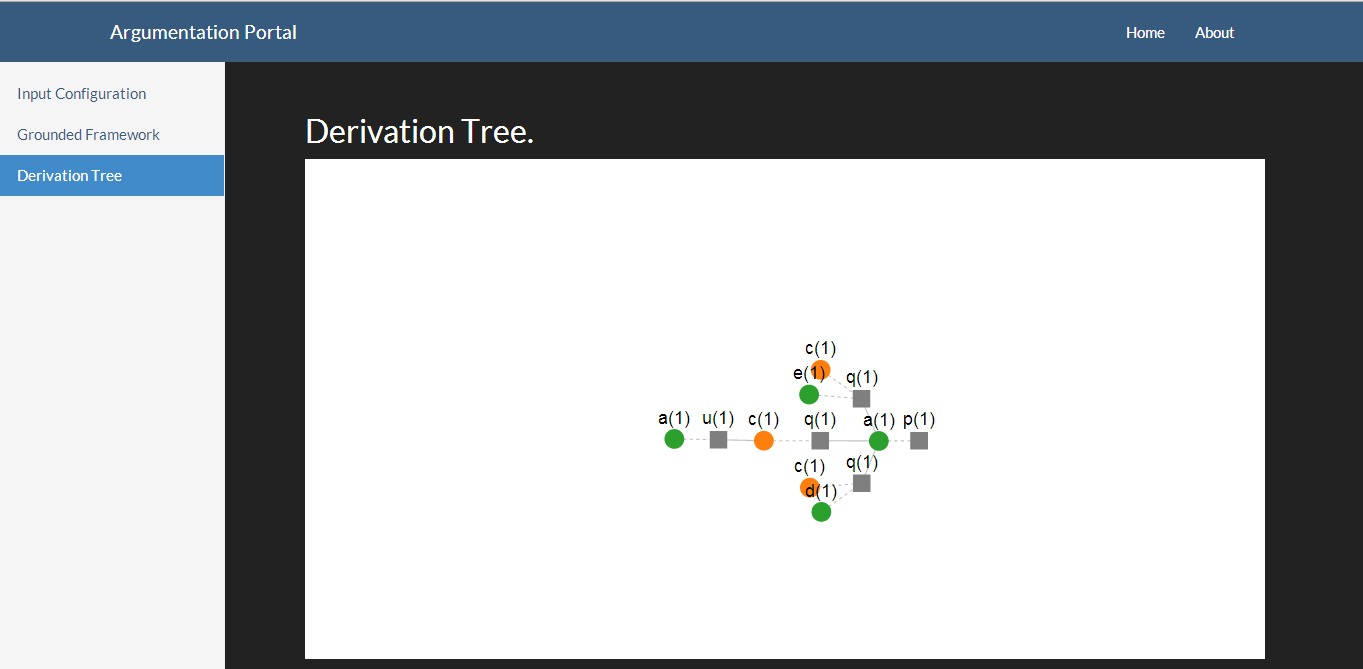
\includegraphics[width=0.8\textwidth]{argumentationOutput.png}
    \caption{Derivation Tree panel.}
    \label{fig:arg_tree}
\end{figure}

\section{Building a Context Free Grammar for the input of the web application.}

We formally defined a Context Free Grammar for the expected user input and built a parser for it. An example of a valid input is given in [TODO].

\begin{Verbatim}[frame=single]

asm(a(X),q(X)){X=1,2;}.
asm(b(X),f(X)){X=1,2;}.
asm(c(X),u(X)){X=1,2;}.
asm(d(X),v(X)){X=1,2;}.
asm(e(X),v(X)){X=1,2;}.
asm(f(X),v(X)){X=1,2;}.

p(X)<-[a(X),u(X)].
q(X)<-[b(X),r(X)].
q(X)<-[c(X),s(X)].
q(X)<-[c(X),t(X)].
u(X)<-[a(X)].
s(X)<-[]{X=1,2;}.
t(X)<-[d(X)].
t(X)<-[e(X)].

\end{Verbatim}

In section [TODO] we elaborate on the semantics of our input language, along with how the parser forced the validity of the user's input.

\section{Grounding a framework over a domain.}

We then extended the language to allow for the specification of a domain over which assumptions, contraries or rules of our framework are valid. In example [TODO] we see how the notation is used to define a domain and the viable variable values.

\begin{Verbatim}[frame=single]
asm(a(X,Y),b(X)){X=1,2,3;Y=a,b;}.
b(X)<-[]{X=1;}.
\end{Verbatim}

We also built a grounder that grounds the framework over the domain specified by the user. The grounder acts as a pre-processing step and allows us to generate the grounded version of our framework as in example [TODO]

\begin{Verbatim}[frame=single]
asm(a(1,a),b(1)). asm(a(1,b),b(1)).
asm(a(2,a),b(2)). asm(a(2,b),b(2)).
asm(a(3,a),b(3)). asm(a(3,b),b(3)).

b(1)<-[].
\end{Verbatim}

An overview of the impementation of the grounder is provided in section [TODO]

\section{Implementing derivations using Ideal Semantics.}

Using the existing implementation of the admissible based dispute derivations in Proxdd, we introduced the necessary functionality that enables us to derive dispute derivations based on ideal semantics. This includes the introduction and correct updating of the ``F'' set , along with the implementation of the Fail(S) check as described in section [TODO]. An example of a successful dispute derivation under the ideal semantics is provided in example [TODO].

\begin{framed}
\begin{exmp} Consider the following assumption based framework:
\\*

\noindent\textbf{R} - includes the following rules:
\\*

\indent	z\textleftarrow a

\indent z\textleftarrow b

\indent y\textleftarrow a

\indent x\textleftarrow d

\indent v\textleftarrow c
\\*

\noindent\textbf{A} = \{a,b,c,d\} and $\bar{a} = z, \bar{b} = y, \bar{c} = x, \bar{d} = v$.

\end{exmp}
\end{framed}

\clearpage

\begin{table}[h]
  \begin{center}
    \begin{tabular}{cccccc}
    \hline
    Step & P     & O         & A     & C     & F         \\ \hline
    1    & \{z\} & \{\}      & \{\}  & \{\}  & \{\}      \\
    2    & \{b\} & \{\}      & \{b\} & \{\}  & \{\}      \\
    3    & \{\}  & \{\{x\}\} & \{b\} & \{\}  & \{\}      \\
    4    & \{z\} & \{\}      & \{b\} & \{a\} & \{\{a\}\} \\
    5    & \{\}  & \{\}      & \{b\} & \{a\} & \{\{a\}\} \\
    6    & \{\}  & \{\}      & \{b\} & \{a\} & \{\}      \\ \hline
    \end{tabular}
    \caption {Example of IB-derivation of example [TODO]}
  \end{center}
\end{table}

The details of the implementation are explored in section [TODO].